\documentclass[12pt]{article}

\usepackage{graphicx}
\graphicspath{{../plots/}}
\usepackage{caption}
\usepackage{subfigure}

\usepackage[utf8]{inputenc}

\usepackage[%
  backend=bibtex,natbib      % biber or bibtex
 ,style=authoryear
 ,sorting=none
 , dashed=false
]{biblatex}
\addbibresource{references.bib}
\DeclareNameAlias{sortname}{first-last}


\title{Russian Language Sentiment Analysis}
\date{}

\begin{document}

\maketitle

\section{Introduction}

\section{Background}

Sentiment analysis is a discipline within natural language processing, analysing people's opinions, attitudes and emotions towards entities and their attributes, as is expressed in written text \parencite{saTextbook}.

Here, the term entity can represent products or services, organisations, events or issues, as well as a host of other THINGS that exist within the world of which people can hold opinions and have attitudes towards.

Sentiment analysis has wide ranging commercial application, as businesses and organisations can leverage consumer opinions to make more accurate decisions regarding their product or service \parencite{deepSAreview}.

For organisations such as governments or local councils, sentiment analysis offers an opportunity to understand public opinion of policy, proposed or existing.

A limitation for natural language processing tasks in general is that for the abundance of English language models, curated data sets and applied research, other languages are incredibly under-represented \parencite{parrots, fivebias}.

To analyse non-English language, there are generally two approaches.

The first, as done by \citet{bautin2008international}, is to use machine translation and perform the sentiment analysis on the English translation of the foreign language text.

The efficacy of such a method, clearly, depends also on the accuracy of the machine translation model. For major world languages this technique is widely applicable, but for smaller languages, it is more difficult.

The second method requires the construction of corpora in the target language.
A corpus is a collection of complete and self-contained texts, which contains information consisting of emotional expressions \parencite{chineseSentiment}.

Analysis of population sentiment can be very useful in wartime. A study by \citet{yemenSocial} analysed from social media data of inhabitants of Yemen over a three month period in 2013. The author concluded that sentiment analysis of the social media data alone could be used for evaluation negative sentiment towards violent extremist organisations or for the standing government.

Sentiment analysis of news articles has been used by social science researchers to investigate research questions related to public opinion. APPRAISALTHEORY

News articles are a good source for building a corpus as there is wide ranging sentiment contained within the texts, as well as generally containing a good lexical sample.

In light of recent events regarding the invasion of Ukraine by the Russian Federation, now more than ever there is a visible need for language models to determine sentiment in languages other than English.

An example where this could be applied is to measure the well-being of citizens living in areas of foreign occupation. 

Further, as shown by \citet{fakeNews}, that sentiment analysis can be used as a method of detecting fake news.

\section{Objectives}

The following report details an attempt at sentiment analysis in the Russian language using the second method previously described. That is, by using a Russian language corpus on which to train the model.

The aim of the project is to build a sentiment analysis model that can then predict sentiment from Russian language news sources from the Russian Federation, as well as Ukraine.

The null hypothesis to be tested would therefore be that there is no significant difference in the sentiment of news articles from the two countries.

\section{Methodology}

The training data set to be used consists of 8,263 Russian language news articles with predetermined sentiment labels of either "positive", "negative" and "neutral". A test data set consists of 2056 samples without labels. The data was originally hosted for a Kaggle competition in 2018 \parencite{dataset}.

\subsection{Data Exploration}

An initial exploration of the data was required to later improve model training.

%distribution of word counts in documents

Firstly, summary statistics for number of words per sample were generated. There is an average of 436 words in sample, with a maximum value of 49,039 words. The long-tail of this distribution is visualised in figure \ref{hist1}.

% HISTOGRAM1


\begin{figure}[ht]
\centering     %%% not \center
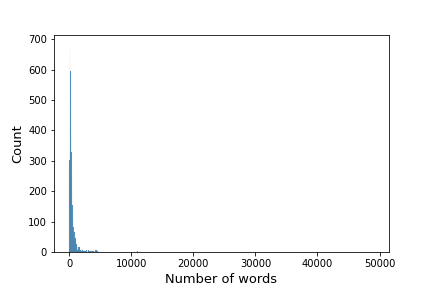
\includegraphics[width=0.65\textwidth]{histogram_original_data1}
\caption{Distribution of the length of texts.}
\label{hist1}
\end{figure}

This means that without any kind of augmentation, the overwhelming majority of samples would need to be padded by two orders of magnitude, vastly increasing the size of input data for the model. A maximum sample length of 500 words was chosen as a filter, leading to training and test data sets of 6284 and 1563 samples, or 76.05\% and 76.02\% of the original data set respectively.

% HISTOGRAM2

\begin{figure}[ht]
\centering     %%% not \center
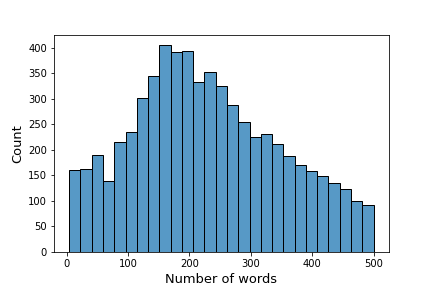
\includegraphics[width=0.65\textwidth]{histogram_original_data2}
\caption{Distribution of the length of texts (500 word maximum).}
\label{hist2}
\end{figure}

As can be seen in figure \ref{hist2}, after generating this subset of the data, the new mean number of words per sample is 209.

%how many unique words in the entire corpus?

An analysis of the entire data set at the word level showed a distinct corpus of 290,028 words, and for the subset 135,779, reducing the total unique word count to 46.82\% of the original data.

%distribution of frequency of words

\subsection{Preprocessing of Data}

In order to prepare the data as an input to the neural networks, it was first converted to lower-case and stripped of punctuation, numbers and special characters.

% REFERENCE LOWERCASING AS BEING VALUABLE IN ANY LANGUAGE

% REFERENCE WHY GET RID OF NUMBERS (maybe embedding later)

Next, a collection of Russian stopwords were removed from the samples. \parencite{russianNLP}

% REFERENCE WHY WE REMOVE STOPWORDS

A final step was taken to stem the words in the samples. This was achieved by use of a Snowball Stemmer by the Natural Language Toolkit package \parencite{nltk}. 

% CITE why we must stem russian language (because of complexity of verb tense, gender, aspect) and case system of nouns and verbs

%what have you done? lowercase CITE, stemming CITE, etc. make sure you have justification for any preprocessing (bonus points for Russian language)

Other preprocessing steps that were initially included but were found to not increase the performance of models were the removal of the most frequent words and the least common words.

%How has the data been processed? Explain the process from going from cleaned textual data to tensors that the model can understand

The summary statistics for the data were then repeated for the reduced cleaned data set, leading to the following observations. 

After filtering again for samples within the limit of 500 words, the number of training examples was 6624, and test 1664, or 80.16\% and 80.93\% of full cleaned data set respectively.

A total of 69.503 unique distinct words existed in the full cleaned data set, with 37,420 in the cleaned data set with the 500 word constraint.

Hence the ratio of words was 53.84\%, which is higher than that found in the original data set. This is to be expected as many rarely used conjugations or cases for particular words will have been retained given their stem is more common.

Once the textual data was in a cleaned state, it was necessary to integer-encode the samples at the word-level. That is, a word-level integer-encoder was used that associates a unique integer value to every unique word in the text (Figure \ref{integer_encoding}).

\begin{figure}[ht]
\centering     %%% not \center
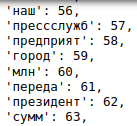
\includegraphics[width=0.35\textwidth]{integer_encoding}
\caption{Integer encoding of Snowball-stemmed vocabulary.}
\label{integer_encoding}
\end{figure}

The final step was to pad the samples so that they were all the same length as neural networks require fixed-dimensional tensor inputs. Each sample was padded with zeros after the end of the text so that it could be represented as a one-dimensional 500-element array.

\subsection{Model Architecture}

% show results for multinomial naive bayes. why?

%**THIS IS A SIGNIFICANT SECTION. DO MUCH RESEARCH** why cnn and rnn? explain your choice. Give references to show where one might be more valuable than the other (again, bonus points for Russian)

% explain the difference between the two

% describe the architecture of the chosen model. GIVE DIAGRAM. GIVE ALL technical details

\section{Experiments}

% What training-test split?

For all neural network experiments undertaken in this project, a number of parameters have been kept constant.

Validation data has been extracted from the training set in a shuffled and stratified manner, with a size of 20\% of the total training set.

All models have been trained using the full vocabulary found in the training set, with a 30-dimensional embedding vector. 

%- What baseline?

%What evaluation metrics?

%build the base rnn model using a single CNN layer with standard

%track training times for all of these models

\subsection{Hyperparameter Selection}

\subsection{Word Embeddings}

\subsection{Transfer-Learning}

\section{Results}

\section{Conclusion}

\printbibliography

\end{document}